A DenseNet121 iteratív tanításának eredményei négy lépésben először 1000 majd 5000 azután 10000 végül pedig 25000 képes halmazon. Ezelet a lépéseket 1k, 5k 10k 25k rövidítésekkel fogom jelölni.

%1K-----------------------------------------------------------------------------
\subsubsection{1k adathalmazon történő tanítás lépései DenseNet121 modellen.}
  \begin{itemize} 
    \item Epoch 1/10 - train: 15/15 [00:03<00:00,  4.48it/s]
    \item Epoch 1: Train loss=4.7857, acc=0.0143 Val loss=4.6317, acc=0.0246
    \item Epoch 2/10 - train: 15/15 [00:02<00:00,  7.29it/s]
    \item Epoch 2: Train loss=3.9205, acc=0.3662 Val loss=4.3919, acc=0.0965
    \item Epoch 3/10 - train: 15/15 [00:02<00:00,  7.36it/s]
    \item Epoch 3: Train loss=3.3158, acc=0.7193 Val loss=4.2184, acc=0.1412
    \item Epoch 4/10 - train: 15/15 [00:02<00:00,  7.23it/s]
    \item Epoch 4: Train loss=2.8105, acc=0.8904 Val loss=4.0804, acc=0.1771
    \item Epoch 5/10 - train: 15/15 [00:02<00:00,  7.37it/s]
    \item Epoch 5: Train loss=2.3650, acc=0.9649 Val loss=3.9495, acc=0.2044
    \item Epoch 6/10 - train: 15/15 [00:02<00:00,  7.30it/s]
    \item Epoch 6: Train loss=1.9764, acc=0.9868 Val loss=3.8034, acc=0.2294
    \item Epoch 7/10 - train: 15/15 [00:02<00:00,  7.26it/s]
    \item Epoch 7: Train loss=1.6406, acc=0.9945 Val loss=3.7104, acc=0.2454
    \item Epoch 8/10 - train: 15/15 [00:02<00:00,  7.33it/s]
    \item Epoch 8: Train loss=1.3594, acc=0.9978 Val loss=3.6529, acc=0.2420
    \item Epoch 9/10 - train: 15/15 [00:02<00:00,  7.36it/s]
    \item Epoch 9: Train loss=1.1032, acc=0.9978 Val loss=3.5557, acc=0.2530
    \item Epoch 10/10 - train: 15/15 [00:02<00:00,  7.29it/s]
    \item Epoch 10: Train loss=0.8931, acc=0.9989 Val loss=3.5198, acc=0.2569
  \end{itemize}

\subsubsection{1k adathalmazon történő tanítás grafikonja DenseNet121 modellen.}
  \begin{figure}[H]
    \centering
    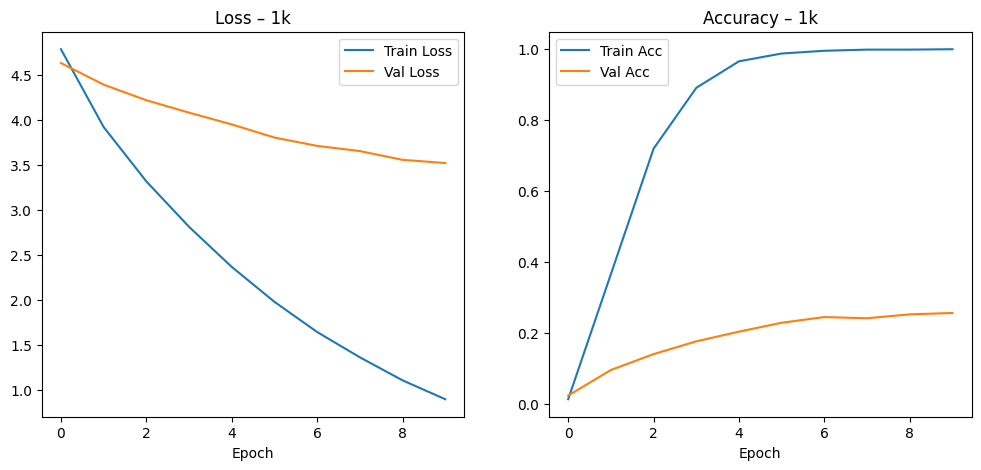
\includegraphics[width=1.0\textwidth]{images/phase03/phase03_DenseNet121_1K_learning_curve.png}
    \caption{1k adathalmazon történő tanítás grafikonja DenseNet121 modellen.}
    \label{fig:phase03_DenseNet121_1K_learning_curve}
  \end{figure}

  \subsubsection{1k adathalmazon történő tanítás eredményei.}
  \begin{center}
    \begin{longtable}{l c}
    \caption{1k tanítás DenseNet121-en.} \label{tab:phase03_DenseNet121_1k} \\
    \toprule
    \textbf{Metrika} & \textbf{Érték} \\
    \midrule
    \endfirsthead
    \toprule
    \textbf{Metrika} & \textbf{Érték} \\
    \midrule
    \endhead
    Top-1 Accuracy & 0.2648 \\
    Top-5 Accuracy & 0.5513 \\
    Precision      & 0.2636 \\
    Recall         & 0.2863 \\
    F1-score       & 0.2542 \\
    Inference time & 25.09 sec \\
    \bottomrule
    \end{longtable}
  \end{center}


%5K-----------------------------------------------------------------------------
\subsubsection{5k adathalmazon történő tanítás lépései DenseNet121 modellen.}
  \begin{itemize} 
    \item Epoch 1/10 - train: 77/77 [00:09<00:00,  8.05it/s]
    \item Epoch 1: Train loss=4.2642, acc=0.1293 Val loss=3.5880, acc=0.2444
    \item Epoch 2/10 - train: 77/77 [00:09<00:00,  8.19it/s]
    \item Epoch 2: Train loss=3.0089, acc=0.4219 Val loss=2.9462, acc=0.3370
    \item Epoch 3/10 - train: 77/77 [00:09<00:00,  7.83it/s]
    \item Epoch 3: Train loss=2.3090, acc=0.5763 Val loss=2.6723, acc=0.3644
    \item Epoch 4/10 - train: 77/77 [00:09<00:00,  8.06it/s]
    \item Epoch 4: Train loss=1.7832, acc=0.7085 Val loss=2.4740, acc=0.4113
    \item Epoch 5/10 - train: 77/77 [00:09<00:00,  8.10it/s]
    \item Epoch 5: Train loss=1.3304, acc=0.8223 Val loss=2.3799, acc=0.4100
    \item Epoch 6/10 - train: 77/77 [00:09<00:00,  8.08it/s]
    \item Epoch 6: Train loss=0.9364, acc=0.9058 Val loss=2.3035, acc=0.4175
    \item Epoch 7/10 - train: 77/77 [00:09<00:00,  8.08it/s]
    \item Epoch 7: Train loss=0.6236, acc=0.9561 Val loss=2.2933, acc=0.4171
    \item Epoch 8/10 - train: 77/77 [00:09<00:00,  8.08it/s]
    \item Epoch 8: Train loss=0.3972, acc=0.9825 Val loss=2.2675, acc=0.4203
    \item Epoch 9/10 - train: 77/77 [00:09<00:00,  8.08it/s]
    \item Epoch 9: Train loss=0.2468, acc=0.9929 Val loss=2.2026, acc=0.4391
    \item Epoch 10/10 - train: 77/77 [00:09<00:00,  8.04it/s]
    \item Epoch 10: Train loss=0.1610, acc=0.9969 Val loss=2.2519, acc=0.4223
  \end{itemize}

\subsubsection{5k adathalmazon történő tanítás grafikonja DenseNet121 modellen.}
  \begin{figure}[H]
    \centering
    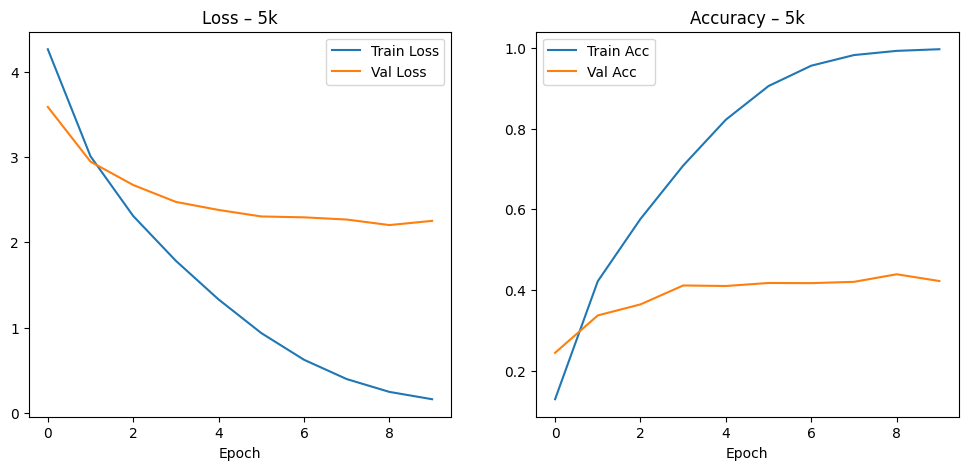
\includegraphics[width=1.0\textwidth]{images/phase03/phase03_DenseNet121_5K_learning_curve.png}
    \caption{5k adathalmazon történő tanítás grafikonja DenseNet121 modellen.}
    \label{fig:phase03_DenseNet121_5K_learning_curve}
  \end{figure}

\subsubsection{5k adathalmazon történő tanítás eredményei.}
\begin{center}
  \begin{longtable}{l c}
  \caption{5k tanítás DenseNet121-en.} \label{tab:phase03_DenseNet121_5k} \\
  \toprule
  \textbf{Metrika} & \textbf{Érték} \\
  \midrule
  \endfirsthead
  \toprule
  \textbf{Metrika} & \textbf{Érték} \\
  \midrule
  \endhead
  Top-1 Accuracy & 0.4309 \\
  Top-5 Accuracy & 0.7514 \\
  Precision      & 0.3957 \\
  Recall         & 0.4491 \\
  F1-score       & 0.4049 \\
  Inference time & 24.87 sec \\
  \bottomrule
  \end{longtable}
\end{center}

%10K-----------------------------------------------------------------------------
\subsubsection{10k adathalmazon történő tanítás lépései DenseNet121 modellen.}
  \begin{itemize} 
    \item Epoch 1/10 - train: 155/155 [00:18<00:00,  8.16it/s]
    \item Epoch 1: Train loss=3.7089, acc=0.2201 Val loss=2.8225, acc=0.3651
    \item Epoch 2/10 - train: 155/155 [00:18<00:00,  8.16it/s]
    \item Epoch 2: Train loss=2.4529, acc=0.4618 Val loss=2.4133, acc=0.4091
    \item Epoch 3/10 - train: 155/155 [00:18<00:00,  8.16it/s]
    \item Epoch 3: Train loss=1.8464, acc=0.5936 Val loss=2.2165, acc=0.4259
    \item Epoch 4/10 - train: 155/155 [00:18<00:00,  8.16it/s]
    \item Epoch 4: Train loss=1.3619, acc=0.7107 Val loss=2.1701, acc=0.4273
    \item Epoch 5/10 - train: 155/155 [00:19<00:00,  8.14it/s]
    \item Epoch 5: Train loss=0.9509, acc=0.8199 Val loss=2.0772, acc=0.4360
    \item Epoch 6/10 - train: 155/155 [00:19<00:00,  8.12it/s]
    \item Epoch 6: Train loss=0.6028, acc=0.9128 Val loss=2.0088, acc=0.4722
    \item Epoch 7/10 - train: 155/155 [00:19<00:00,  8.14it/s]
    \item Epoch 7: Train loss=0.3473, acc=0.9642 Val loss=2.0728, acc=0.4614
    \item Epoch 8/10 - train: 155/155 [00:19<00:00,  8.15it/s]
    \item Epoch 8: Train loss=0.1926, acc=0.9873 Val loss=2.0269, acc=0.4720
    \item Epoch 9/10 - train: 155/155 [00:19<00:00,  8.01it/s]
    \item Epoch 9: Train loss=0.1117, acc=0.9942 Val loss=2.0559, acc=0.4789
    \item Epoch 10/10 - train: 155/155 [00:19<00:00,  8.14it/s]
    \item Epoch 10: Train loss=0.0667, acc=0.9971 Val loss=2.1183, acc=0.4737
  \end{itemize}

\subsubsection{10k adathalmazon történő tanítás grafikonja DenseNet121 modellen.}
  \begin{figure}[H]
    \centering
    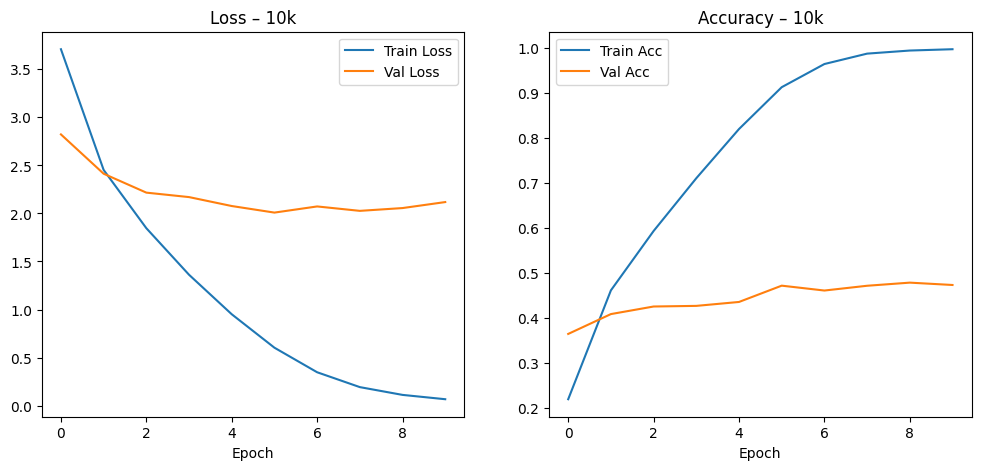
\includegraphics[width=1.0\textwidth]{images/phase03/phase03_DenseNet121_10K_learning_curve.png}
    \caption{10k adathalmazon történő tanítás grafikonja DenseNet121 modellen.}
    \label{fig:phase03_DenseNet121_10K_learning_curve}
  \end{figure}

\subsubsection{10k adathalmazon történő tanítás eredményei.}
  \begin{center}
    \begin{longtable}{l c}
    \caption{10k tanítás DenseNet121-en.} \label{tab:phase03_DenseNet121_10k} \\
    \toprule
    \textbf{Metrika} & \textbf{Érték} \\
    \midrule
    \endfirsthead
    \toprule
    \textbf{Metrika} & \textbf{Érték} \\
    \midrule
    \endhead
    Top-1 Accuracy & 0.4793 \\
    Top-5 Accuracy & 0.7849 \\
    Precision      & 0.4390 \\
    Recall         & 0.5065 \\
    F1-score       & 0.4542 \\
    Inference time & 25.02 sec \\
    \bottomrule
    \end{longtable}
  \end{center}

%25K-----------------------------------------------------------------------------
\subsubsection{25k adathalmazon történő tanítás lépései DenseNet121 modellen.}
  \begin{itemize} 
    \item Epoch 1/10 - train: 391/391 [00:47<00:00,  8.23it/s]
    \item Epoch 1: Train loss=3.0551, acc=0.3175 Val loss=2.2636, acc=0.4364
    \item Epoch 2/10 - train: 391/391 [00:47<00:00,  8.26it/s]
    \item Epoch 2: Train loss=1.9269, acc=0.5255 Val loss=1.9442, acc=0.4782
    \item Epoch 3/10 - train: 391/391 [00:47<00:00,  8.26it/s]
    \item Epoch 3: Train loss=1.4036, acc=0.6477 Val loss=1.8720, acc=0.4847
    \item Epoch 4/10 - train: 391/391 [00:47<00:00,  8.21it/s]
    \item Epoch 4: Train loss=0.9916, acc=0.7555 Val loss=1.7271, acc=0.5304
    \item Epoch 5/10 - train: 391/391 [00:47<00:00,  8.17it/s]
    \item Epoch 5: Train loss=0.6593, acc=0.8449 Val loss=1.8182, acc=0.5182
    \item Epoch 6/10 - train: 391/391 [00:47<00:00,  8.22it/s]
    \item Epoch 6: Train loss=0.3995, acc=0.9168 Val loss=1.8705, acc=0.5201
    \item Epoch 7/10 - train: 391/391 [00:47<00:00,  8.24it/s]
    \item Epoch 7: Train loss=0.2486, acc=0.9538 Val loss=1.9755, acc=0.5161
    \item Epoch 8/10 - train: 391/391 [00:47<00:00,  8.21it/s]
    \item Epoch 8: Train loss=0.1689, acc=0.9703 Val loss=2.0438, acc=0.5145
    \item Epoch 9/10 - train: 391/391 [00:47<00:00,  8.22it/s]
    \item Epoch 9: Train loss=0.1524, acc=0.9730 Val loss=2.1919, acc=0.5052
    \item Epoch 10/10 - train: 391/391 [00:47<00:00,  8.20it/s]
    \item Epoch 10: Train loss=0.1022, acc=0.9829 Val loss=2.0833, acc=0.5307
  \end{itemize}

\subsubsection{25k adathalmazon történő tanítás grafikonja DenseNet121 modellen.}
  \begin{figure}[H]
    \centering
    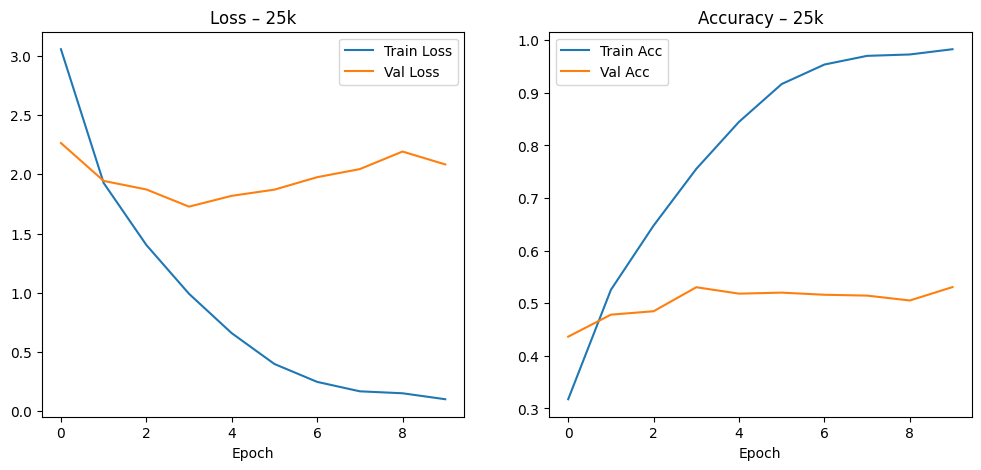
\includegraphics[width=1.0\textwidth]{images/phase03/phase03_DenseNet121_25K_learning_curve.png}
    \caption{25k adathalmazon történő tanítás grafikonja DenseNet121 modellen.}
    \label{fig:phase03_DenseNet121_25K_learning_curve}
  \end{figure}

\subsubsection{25k adathalmazon történő tanítás eredményei.}
  \begin{center}
    \begin{longtable}{l c}
    \caption{25k tanítás DenseNet121-en.} \label{tab:phase03_DenseNet121_25k} \\
    \toprule
    \textbf{Metrika} & \textbf{Érték} \\
    \midrule
    \endfirsthead
    \toprule
    \textbf{Metrika} & \textbf{Érték} \\
    \midrule
    \endhead
    Top-1 Accuracy & 0.5366 \\
    Top-5 Accuracy & 0.8207 \\
    Precision      & 0.5003 \\
    Recall         & 0.5739 \\
    F1-score       & 0.5171 \\
    Inference time & 24.71 sec \\
    \bottomrule
    \end{longtable}
  \end{center}

\subsubsection{DenseNet121 iteratív tanítás összefoglaló}
  \begin{center}
    \begin{longtable}{lllllll}
    \caption{Összehasonlító táblázat a DenseNet121 iteratív tanításáról.}\label{tab:phase3_DenseNet121_summary_table}\\
    \toprule
    Minta & Top-1 & Top-5 & Precision & Recall & F1 & Time(s) \\
    \midrule
    \endfirsthead
    \toprule
    Minta & Top-1 & Top-5 & Precision & Recall & F1 & Time(s) \\
    \midrule
    \endhead
    1k & 0.2648 & 0.5513 & 0.2636 & 0.2863 & 0.2542 & 25.09 \\
    5k & 0.4309 & 0.7514 & 0.3957 & 0.4491 & 0.4049 & 24.87 \\
    10k & 0.4793 & 0.7849 & 0.4390 & 0.5065 & 0.4542 & 25.02 \\
    25k & 0.5366 & 0.8207 & 0.5003 & 0.5739 & 0.5171 & 24.71 \\
    \bottomrule
    \end{longtable}
  \end{center}
  

  \subsubsection{Összehasonlító grafikon a DenseNet121 iteratív tanításáról.}
  \begin{figure}[H]
    \centering
    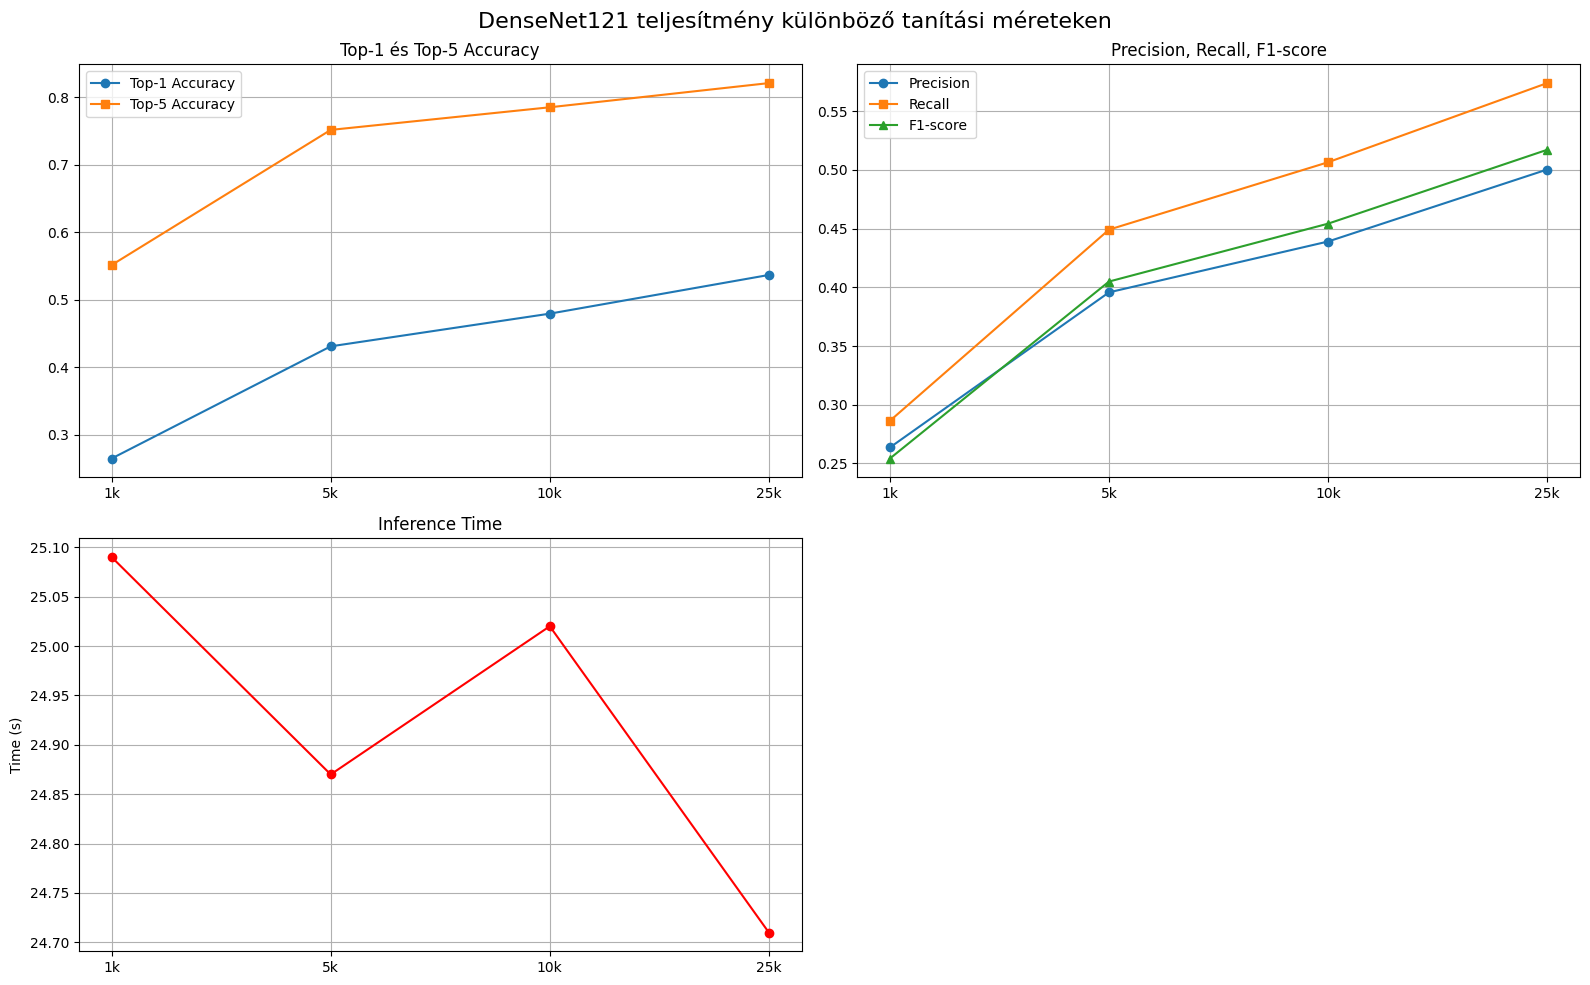
\includegraphics[width=1.0\textwidth]{images/phase03/phase03_DenseNet121_summary_curve.png}
    \caption{Összehasonlító grafikon a DenseNet121 iteratív tanításáról.}
    \label{fig:phase03_DenseNet121_summary_curve}
  \end{figure}

  \subsubsection{Összehasonlító grafikon a DenseNet121 iteratív tanításáról 10 EPOCH-on keresztül.}
  \begin{figure}[H]
    \centering
    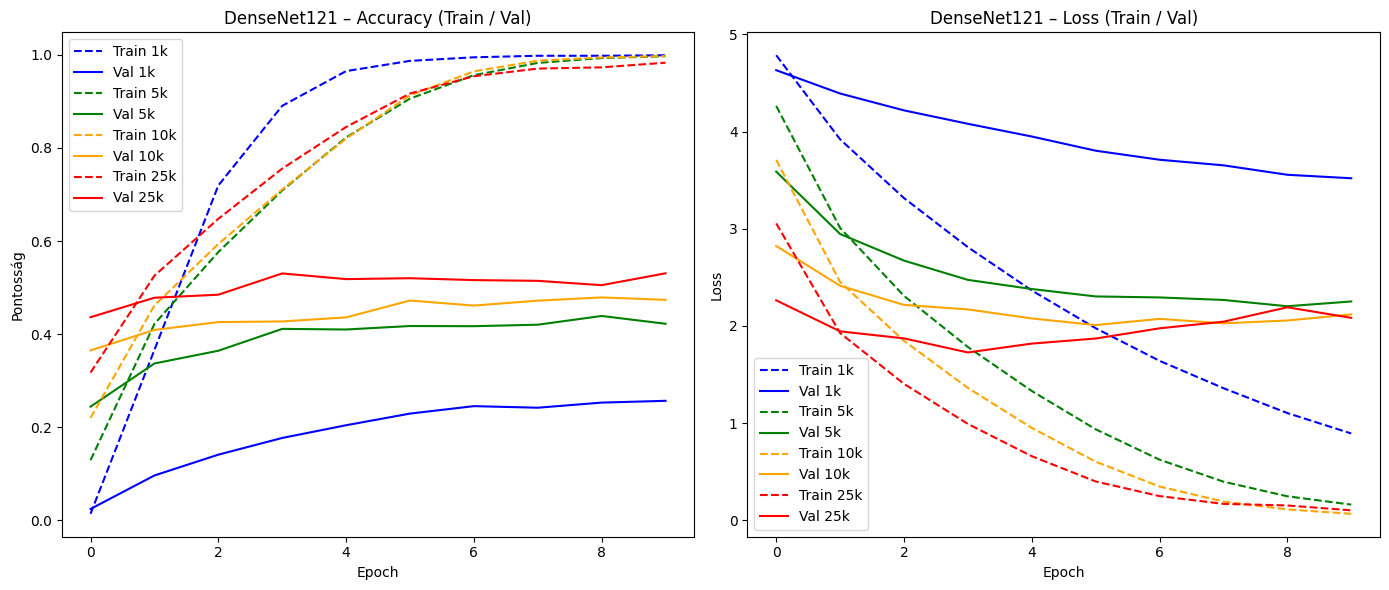
\includegraphics[width=1.0\textwidth]{images/phase03/phase03_DenseNet121_learning_summary_curve.png}
    \caption{Összehasonlító grafikon a DenseNet121 iteratív tanításáról 10 EPOCH-on keresztül.}
    \label{fig:phase03_DenseNet121_learning_summary_curve}
  \end{figure}

  \subsubsection{Összehasonlító Confusion Matrix a DenseNet121 iteratív tanításáról.}
  \begin{figure}[H]
    \centering
    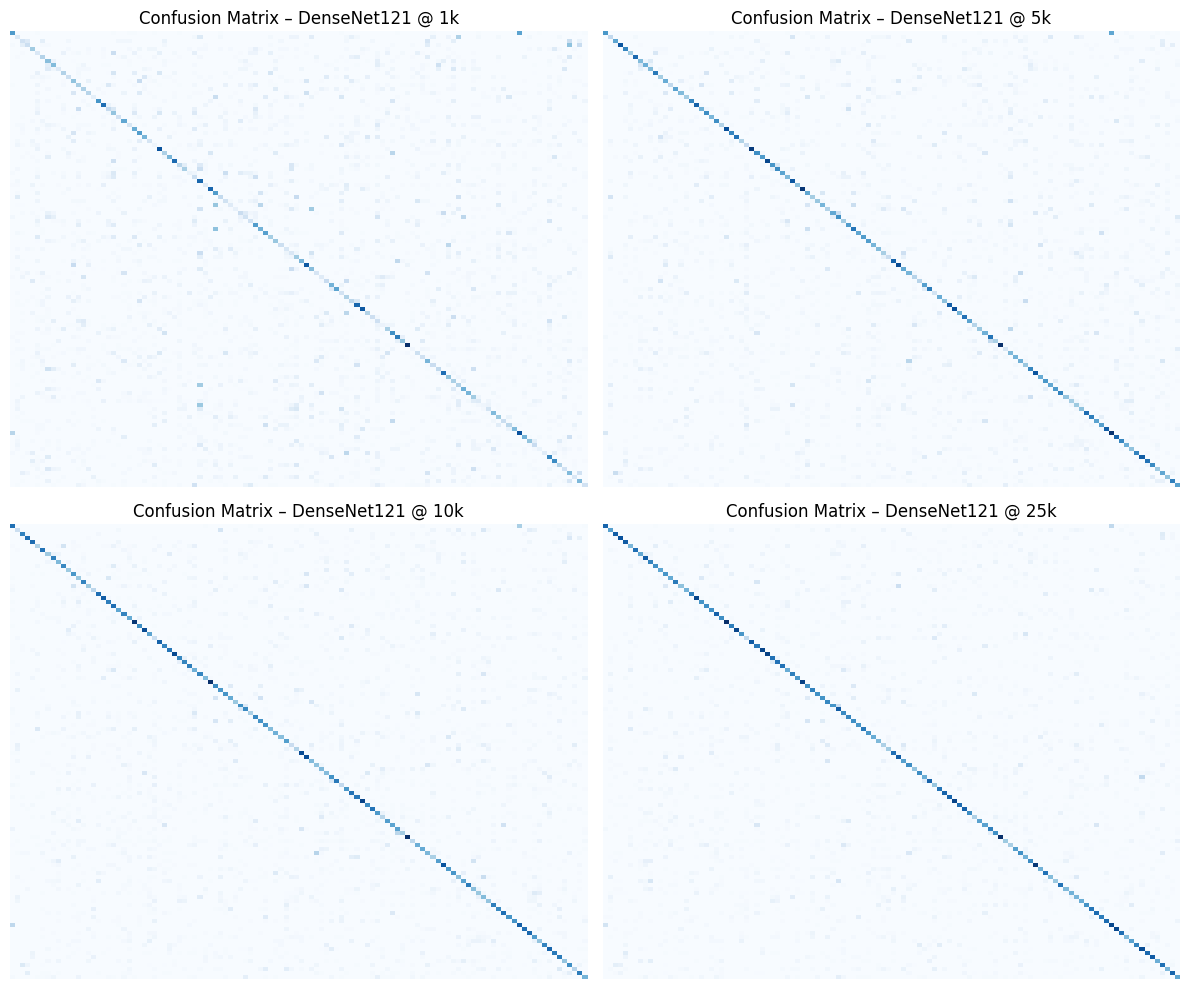
\includegraphics[width=1.0\textwidth]{images/phase03/phase03_DenseNet121_Confusion_Matrix_summary_curve.png}
    \caption{Összehasonlító Confusion Matrix a DenseNet121 iteratív tanításáról 10 EPOCH-on keresztül.}
    \label{fig:phase03_DenseNet121_Confusion_Matrix_summary_curve}
  \end{figure}